\documentclass[english,,man,floatsintext]{apa6}
\usepackage{lmodern}
\usepackage{amssymb,amsmath}
\usepackage{ifxetex,ifluatex}
\usepackage{fixltx2e} % provides \textsubscript
\ifnum 0\ifxetex 1\fi\ifluatex 1\fi=0 % if pdftex
  \usepackage[T1]{fontenc}
  \usepackage[utf8]{inputenc}
\else % if luatex or xelatex
  \ifxetex
    \usepackage{mathspec}
  \else
    \usepackage{fontspec}
  \fi
  \defaultfontfeatures{Ligatures=TeX,Scale=MatchLowercase}
    \setmainfont[]{Times New Roman}
\fi
% use upquote if available, for straight quotes in verbatim environments
\IfFileExists{upquote.sty}{\usepackage{upquote}}{}
% use microtype if available
\IfFileExists{microtype.sty}{%
\usepackage{microtype}
\UseMicrotypeSet[protrusion]{basicmath} % disable protrusion for tt fonts
}{}
\usepackage{hyperref}
\hypersetup{unicode=true,
            pdftitle={Context-specific attentional sampling: Intentional control as pre-requisite for contextual control.},
            pdfauthor={Nicholaus P. Brosowsky~\& Matthew J. C. Crump},
            pdfkeywords={Attention, Attentional sampling, Contextual control, Awareness,
Intention},
            pdfborder={0 0 0},
            breaklinks=true}
\urlstyle{same}  % don't use monospace font for urls
\ifnum 0\ifxetex 1\fi\ifluatex 1\fi=0 % if pdftex
  \usepackage[shorthands=off,main=english]{babel}
\else
  \usepackage{polyglossia}
  \setmainlanguage[]{english}
\fi
\usepackage{graphicx,grffile}
\makeatletter
\def\maxwidth{\ifdim\Gin@nat@width>\linewidth\linewidth\else\Gin@nat@width\fi}
\def\maxheight{\ifdim\Gin@nat@height>\textheight\textheight\else\Gin@nat@height\fi}
\makeatother
% Scale images if necessary, so that they will not overflow the page
% margins by default, and it is still possible to overwrite the defaults
% using explicit options in \includegraphics[width, height, ...]{}
\setkeys{Gin}{width=\maxwidth,height=\maxheight,keepaspectratio}
\IfFileExists{parskip.sty}{%
\usepackage{parskip}
}{% else
\setlength{\parindent}{0pt}
\setlength{\parskip}{6pt plus 2pt minus 1pt}
}
\setlength{\emergencystretch}{3em}  % prevent overfull lines
\providecommand{\tightlist}{%
  \setlength{\itemsep}{0pt}\setlength{\parskip}{0pt}}
\setcounter{secnumdepth}{0}
% Redefines (sub)paragraphs to behave more like sections
\ifx\paragraph\undefined\else
\let\oldparagraph\paragraph
\renewcommand{\paragraph}[1]{\oldparagraph{#1}\mbox{}}
\fi
\ifx\subparagraph\undefined\else
\let\oldsubparagraph\subparagraph
\renewcommand{\subparagraph}[1]{\oldsubparagraph{#1}\mbox{}}
\fi

%%% Use protect on footnotes to avoid problems with footnotes in titles
\let\rmarkdownfootnote\footnote%
\def\footnote{\protect\rmarkdownfootnote}


  \title{Context-specific attentional sampling: Intentional control as
pre-requisite for contextual control.}
    \author{Nicholaus P. Brosowsky\textsuperscript{1}~\& Matthew J. C.
Crump\textsuperscript{2}}
    \date{}
  
\shorttitle{Context-specific attentional sampling}
\affiliation{
\vspace{0.5cm}
\textsuperscript{1} The Graduate Center of the City University of New York\\\textsuperscript{2} Brooklyn College of the City University of New York}
\keywords{Attention, Attentional sampling, Contextual control, Awareness, Intention}
\usepackage{csquotes}
\usepackage{upgreek}
\captionsetup{font=singlespacing,justification=justified}

\usepackage{longtable}
\usepackage{lscape}
\usepackage{multirow}
\usepackage{tabularx}
\usepackage[flushleft]{threeparttable}
\usepackage{threeparttablex}

\newenvironment{lltable}{\begin{landscape}\begin{center}\begin{ThreePartTable}}{\end{ThreePartTable}\end{center}\end{landscape}}

\makeatletter
\newcommand\LastLTentrywidth{1em}
\newlength\longtablewidth
\setlength{\longtablewidth}{1in}
\newcommand{\getlongtablewidth}{\begingroup \ifcsname LT@\roman{LT@tables}\endcsname \global\longtablewidth=0pt \renewcommand{\LT@entry}[2]{\global\advance\longtablewidth by ##2\relax\gdef\LastLTentrywidth{##2}}\@nameuse{LT@\roman{LT@tables}} \fi \endgroup}


\usepackage{setspace}\doublespacing
\newenvironment{zeroindent} {\par\setlength{\parindent}{0pt}} {\par}
\setlength{\parskip}{0pt}
\raggedbottom

\authornote{

Correspondence concerning this article should be addressed to Nicholaus
P. Brosowsky, The Graduate Center, CUNY, 365 5th Ave, New York, NY
10016. E-mail:
\href{mailto:nbrosowsky@gradcenter.cuny.edu}{\nolinkurl{nbrosowsky@gradcenter.cuny.edu}}}

\abstract{
Recent work suggests that environmental cues associated with previous
attentional control settings can rapidly and involuntarily adjust
attentional priorities. The current study tests predictions from
adaptive-learning and memory-based theories of contextual control about
the role of intentions for setting attentional priorities. To extend the
empirical boundaries of contextual control phenomena, and to determine
whether theoretical principles of contextual control are generalizable
we used a novel bi-dimensional stimulus sampling task. Subjects viewed
briefly presented arrays of letters and colors presented above or below
fixation, and identified specific stimuli according to a dimensional
(letter or color) and positional cue. Location was predictive of the
cued dimension, but not the position or identity. In contrast to
previous findings, contextual control failed to develop through
automatic, adaptive-learning processes. Instead, previous experience
with intentionally changing attentional sampling priorities between
different contexts was required for contextual control to develop.


}

\begin{document}
\maketitle

\section{Introduction}\label{introduction}

Attentional control refers to processes that alter priorities for
selecting relevant versus irrelevant information during task
performance. Although attentional priorities are widely understood to be
set in an effortful intentional fashion (Posner \& Snyder, 1975), they
may also be set in a cue-driven fashion. For example, research across
paradigms in attention suggests that contextual cues can trigger the
automatic retrieval and reinstatement of attentional control settings
previously used in those contexts in the past (for reviews, see Bugg \&
Crump, 2012; Cosman \& Vecera, 2013; Egner, 2008). The present
experiments contribute to this body of work by showing new evidence of
location-based contextual control over priorities for sampling from
briefly presented bi-dimensional (e.g., letters and colors),
multi-element displays. More important, across experiments we find that
contextual control over sampling in this procedure depends on an
intentional learning phase where subjects explicitly deploy different
sampling strategies in different location contexts. These findings
contrast with several existing demonstrations of contextual control that
do not appear to depend on intentional processing, and they are also not
well explained by accounts of contextual control that posit a role for
learning processes that automatically adapt to the statistics of the
environment. To set the stage for the present work, we briefly review
the range of evidence for contextual control, what is known about the
roles of awareness and intention in acquiring contextual control, and
how these issues are treated among major theories of contextual control.

Demonstrations of contextual control over attentional priorities have
been observed in procedures tapping different aspects of attention. For
example, repeating the configuration of distractors in visual search
facilitates target detection (Chun, 2000; Chun \& Jiang, 1998). Stroop
interference reflecting priorities for processing color versus word
information is modulated by contextual cues (location, shape, font)
associated with different proportions of congruent and incongruent items
(Crump \& Milliken, 2009; Crump, Gong, \& Milliken, 2006; Crump,
Vaquero, \& Milliken, 2008). Flanker interference reflecting priorities
for selecting a target in space from nearby distractors is also
modulated by contexts associated with different proportions of congruent
and incongruent items (Corballis \& Gratton, 2003; Crump, 2016; King,
Korb, \& Egner, 2012). Similarly, task-switching costs reflecting
task-specific attentional priorities can be modulated by contextual cues
associated with specific tasks (Mayr \& Bryck, 2007), and different
proportions of switch and repeat trials (Crump \& Logan, 2010).
Attention capture by salient feature singletons (Cosman \& Vecera, 2013;
see also, Le Pelley, Vadillo, \& Luque, 2013) can also be modulated by
context cues (e.g., visual scenes) associated with differing attentional
sets. Related findings showing cue-driven control over the setting of
attentional priorities can be found in negative priming (Milliken,
Thomson, Bleile, MacLellan, \& Giammarco, 2012), priming of pop-out
(Thomson \& Milliken, 2013), and masked-priming (Heinemann, Kunde, \&
Kiesel, 2009; Panadero, Castellanos, \& Tudela, 2015; Reuss, Desender,
Kiesel, \& Kunde, 2014). The present experiments borrow techniques from
demonstrations of contextual control over congruency effects in classic
selective attention procedures like Stroop or flanker; so, we discuss
those demonstrations more closely as a venue for reviewing the roles of
awareness and intention in contextual control.

Interference tasks like Stroop (1935) and flanker (B. A. Eriksen \&
Eriksen, 1974) require subjects to identify a target dimension while
ignoring a distractor dimension. For example, in the Stroop task (for a
review, see MacLeod, 1991) subjects identify the ink-color of a written
color word, and performance is typically worse when the distracting word
is incongruent (e.g., the word RED is printed in blue) than congruent
(e.g., the word RED is printed in red) with the required response. The
size of this difference, termed the congruency effect, is taken as an
index of selective attention: larger differences show failures to
prevent distractors from influencing performance, and smaller
differences show success in preventing distractors from influencing
performance. Proportion congruent manipulations modulate the size of
congruency effects, and are a common tool for measuring control
processes that set attentional priorities for target and distractor
processing (for a review, see Bugg \& Crump, 2012). Proportion congruent
manipulations vary the relative proportion of congruent and incongruent
items in a task. Generally, congruency effects are larger in blocks of
trials that have a higher than lower proportion of congruent items
(Logan \& Zbrodoff, 1979).

Contextual control over congruency effects has been shown using
context-specific proportion congruent manipulations. For example, Crump
et al. (2006) presented Stroop items in a randomized intermixed fashion
in one of two locations that were associated with a high or low
proportion of congruent items. In this design, subjects were unable to
predict whether an upcoming trial would be congruent or incongruent, or
whether an item would appear in a location that was high or low
proportion congruent. Nevertheless, larger congruency effects were found
for the items in the high than low proportion congruent locations. This
finding is consistent with contextual control over attentional sets,
whereby rapid, online processing of location cues associated with
different levels of proportion congruent trigger adjustments to
priorities for filtering color and word dimensions of a current item.
The CSPC effect has been reported several times in Stroop (Bugg, Jacoby,
\& Toth, 2008; Crump \& Milliken, 2009; Crump et al., 2008), and flanker
tasks (Corballis \& Gratton, 2003; Wendt \& Luna-Rodriguez, 2009; Wendt,
Kluwe, \& Vietze, 2008).

The interpretation that CSPC effects reflect automatic contextual
control depends on a subject's state of awareness and possible intention
to set attentional priorities by context. We use awareness to refer to
explicit knowledge of the proportion congruent manipulation, the source
of conflict, or the presence of contextual cues. We use intention to
refer to a deliberate route for setting attentional priorities. Subjects
could become aware of the CSPC manipulation, that attentional
requirements vary by context, and then deliberately set attentional
priorities separately for each context. Intentional control could
prepare two different strategies in advance, or rapidly shift
attentional priorities in response to the presentation of a context cue.
Either way, the CSPC effect would not provide clear evidence for an
automatic cue-driven influence over attentional priorities.
Additionally, subjects could be aware of the CSPC manipulation, but
decide not to intentionally assign different attentional priorities
between contexts. In this case, intentional control would not explain
CSPC effects, although awareness could play a role in learning about
predictive cues. Subjects could also be unaware of the CSPC
manipulation, and presumably for that reason would not intentionally set
attentional priorities in a context-specific fashion that would produce
consistent CSPC effects. Here, CSPC effects would be more consistent
with an automatic, cue-driven influence over the setting of attentional
priorities.

Awareness of the CSPC manipulation has been assessed by
post-experimental questionnaires. All of the studies measuring awareness
showed that subjects could not accurately report the relative
proportions of congruent items between contexts (Crump \& Logan, 2010;
Crump et al., 2006; Gough, Garcia, Torres-Quesada, \& Milliken, 2014;
King et al., 2012; Sarmiento, Shore, Milliken, \& Sanabria, 2012). A few
studies have also manipulated awareness. Crump et al. (2008) for
example, tested whether awareness of the CSPC manipulation would be
sufficient for producing contextual control using shape cues, which were
previously found to be an ineffective cue for observing CSPC effects
(Crump et al., 2006). Subjects were informed about the CSPC
manipulation, encouraged to use shape-specific attentional control
strategies, and signed a statement acknowledging they understood the
instructions. CSPC effects for shape cues were not observed, and
subjects were unable to accurately complete the post-experiment
awareness questionnaire. Awareness of conflict between the relevant and
irrelevant dimensions has also been assessed as a pre-requisite for CSPC
effects. For example, CSPC effects can be produced in masked-prime
procedures where subjects are not aware of the source of response
conflict (Heinemann et al., 2009; Panadero et al., 2015; Reuss et al.,
2014; but see, Schouppe, Ferrerre, Van Opstal, Braem, \& Notebaert,
2014). Reuss et al. (2014) embedded the contextual cue within the masked
prime and found CSPC effects even when the prime was below a perceptible
threshold. Taken together, these studies suggest that awareness of the
CSPC manipulation, source of response conflict, and in one case the
presence of a contextual cue, are not prerequisites for contextual
control; they also suggest that CSPC effects are not driven by
intentional means.

Process theories of CSPC effects and contextual control phenomena
generally do not invoke awareness or intention as pre-requisites for
acquiring or displaying cue-driven control after learning. We review two
general classes of theories termed adaptive learning and memory-based
accounts.

Adaptive learning theories explain contextual control in terms of
automatic learning processes sensitive to the statistics of the
environment, and have a long history in attention (Moray \& Fitter,
1973) and associative learning (Mackintosh, 1975) theory. Generally
speaking, adaptive learning processes update attentional priorities in
response to errors, such that future errors are minimized (Kruschke,
1992, 2001, 2003, 2010). Similar approaches using response conflict
signals (Botvinick, Braver, Barch, Carter, \& Cohen, 2001) have modeled
item-specific proportion congruent effects (Blais, Harris, Guerrero, \&
Bunge, 2012), and could account for CSPC effects if items in each
context were represented individually. Verguts and Notebaert (2008,
2009) also showed that a Hebbian learning rule could further control how
conflict signals update attentional priorities. More generally,
experienced conflict, actual errors, and error estimates all represent
learning signals by which performance could potentially be optimized
Verguts and Notebaert (2008). According to these models, the
prerequisites for acquiring contextual control include the presence of a
learning signal, and the presence of statistical regularities among
environment cues that can direct optimization. Awareness of
environmental regularities, or intentional control of attentional
prioritization are not required for contextual control.

Memory-based theories explain contextual control by cue-driven retrieval
and reinstatement of prior attentional priorities (Crump, 2016; Crump \&
Milliken, 2009; Crump et al., 2006, 2008). Memory traces store the
perceptual details of specific experiences and the attentional
priorities for information processing assigned during those experiences.
In this way, cues in the present moment can retrieve similar instances
from memory and reinstate the attentional priorities used in the past to
update attentional priorities in the present. Memory-driven theories can
be flexible with respect to the roles of awareness and intention. The
critical assumption of the memory account is that subjects possess
memory traces that code different attentional priorities for different
contexts. The theory suggests that context-specific attentional
priorities could be obtained through various means, including adaptive
learning, or intentional control at the level of items or contexts.
First, adaptive learning processes could work in concert with memory and
provide the mechanism for changing attentional priorities in a
context-specific fashion. Second, memory processes could produce
contextual control through generalization of attentional priorities for
specific items that vary between contexts. For example, subjects may
intentionally modify attentional priorities for specific items to
maximize speed and accuracy, and item-specific priorities associated to
and retrieved by context cues could generalize to other items appearing
in those contexts. Finally, memory processes could rely on initial
awareness of context-specific differences in attentional requirements,
and subsequent intentional control to assign different attentional
priorities between contexts. In this way, memory would be populated with
instances that code context-specific attentional priorities, which could
then be retrieved in an automatic cue-driven fashion.

Taking stock, research into contextual control has generated numerous
empirical demonstrations and some process theories with generalizable
principles for explaining how cues acquire the ability to adjust
attentional priorities during performance. A broad aim of the present
experiments was to evaluate the generalizability of predictions from
adaptive-learning and memory-based theories, especially with respect to
intentional control. Our approach was to examine the acquisition of
contextual control in a novel task that required subjects to prioritize
sampling from one of two dimensions (letters or colors) in briefly
presented multi-element displays. The use of a novel task had the dual
benefits of assessing whether theoretical predictions are
paradigm-specific or paradigm-general, as well as identifying new
empirical boundaries for contextual control phenomena. The major finding
across experiments is that contextual control in our task depends on
intentional control. That is, previous experience with intentionally
changing attentional sampling priorities between different contexts is a
pre-requisite for contextual control over sampling from briefly
presented displays.

\section{Experiment 1}\label{experiment-1}

Our task was similar to Sperling's (1960) partial report paradigm where
complex visual displays are presented followed by instructions
indicating target selection criterion. We used bi-dimensional displays
containing letter and colors, which allow for independent, selective
processing (Bundesen, Kyllingsbæk, \& Larsen, 2003; Kyllingsbæk \&
Bundesen, 2007). Each display contained a row of four different letters
inside four uniquely colored squares. Displays were briefly presented
(300 ms) followed by a task cue to report the identity of the letter or
color that appeared in one of the squares (see Figure
\ref{fig:figure1}).

Borrowing from the location-based CSPC manipulation, our displays
appeared in one of two locations above or below the fixation, and
location was predictive of the identification task (color vs.~letter),
but not the position or identity of the items in each display.
Specifically, one location involved 75\% color and 25\% letter
identification trials, and the other location involved 75\% letter and
25\% color identification trials, so the location predicted the current
task with 75\% validity. We use the term valid to refer to trials where
each identification task appeared in its likely location (75\%), and the
term invalid to refer to trials where each identification task appeared
in its unlikely location (25\%).

Thus, we created experimental conditions that have produced contextual
control over congruency effects in Stroop and flanker. We assumed these
conditions would also produce location-based control over attentional
priorities for sampling from distinct dimensions in briefly presented
visual displays. Specifically, we expected that identification accuracy
would be higher for both letter and color targets when displayed in
their respective valid than invalid locations. We did not inform
subjects that location was predictive of the identification task, and we
expected that subjects would not become aware of the manipulation. From
the perspective of adaptive learning theories of contextual control, we
assumed that attentional priorities would shift automatically in
response to errors or conflict.

\begin{figure}
\centering
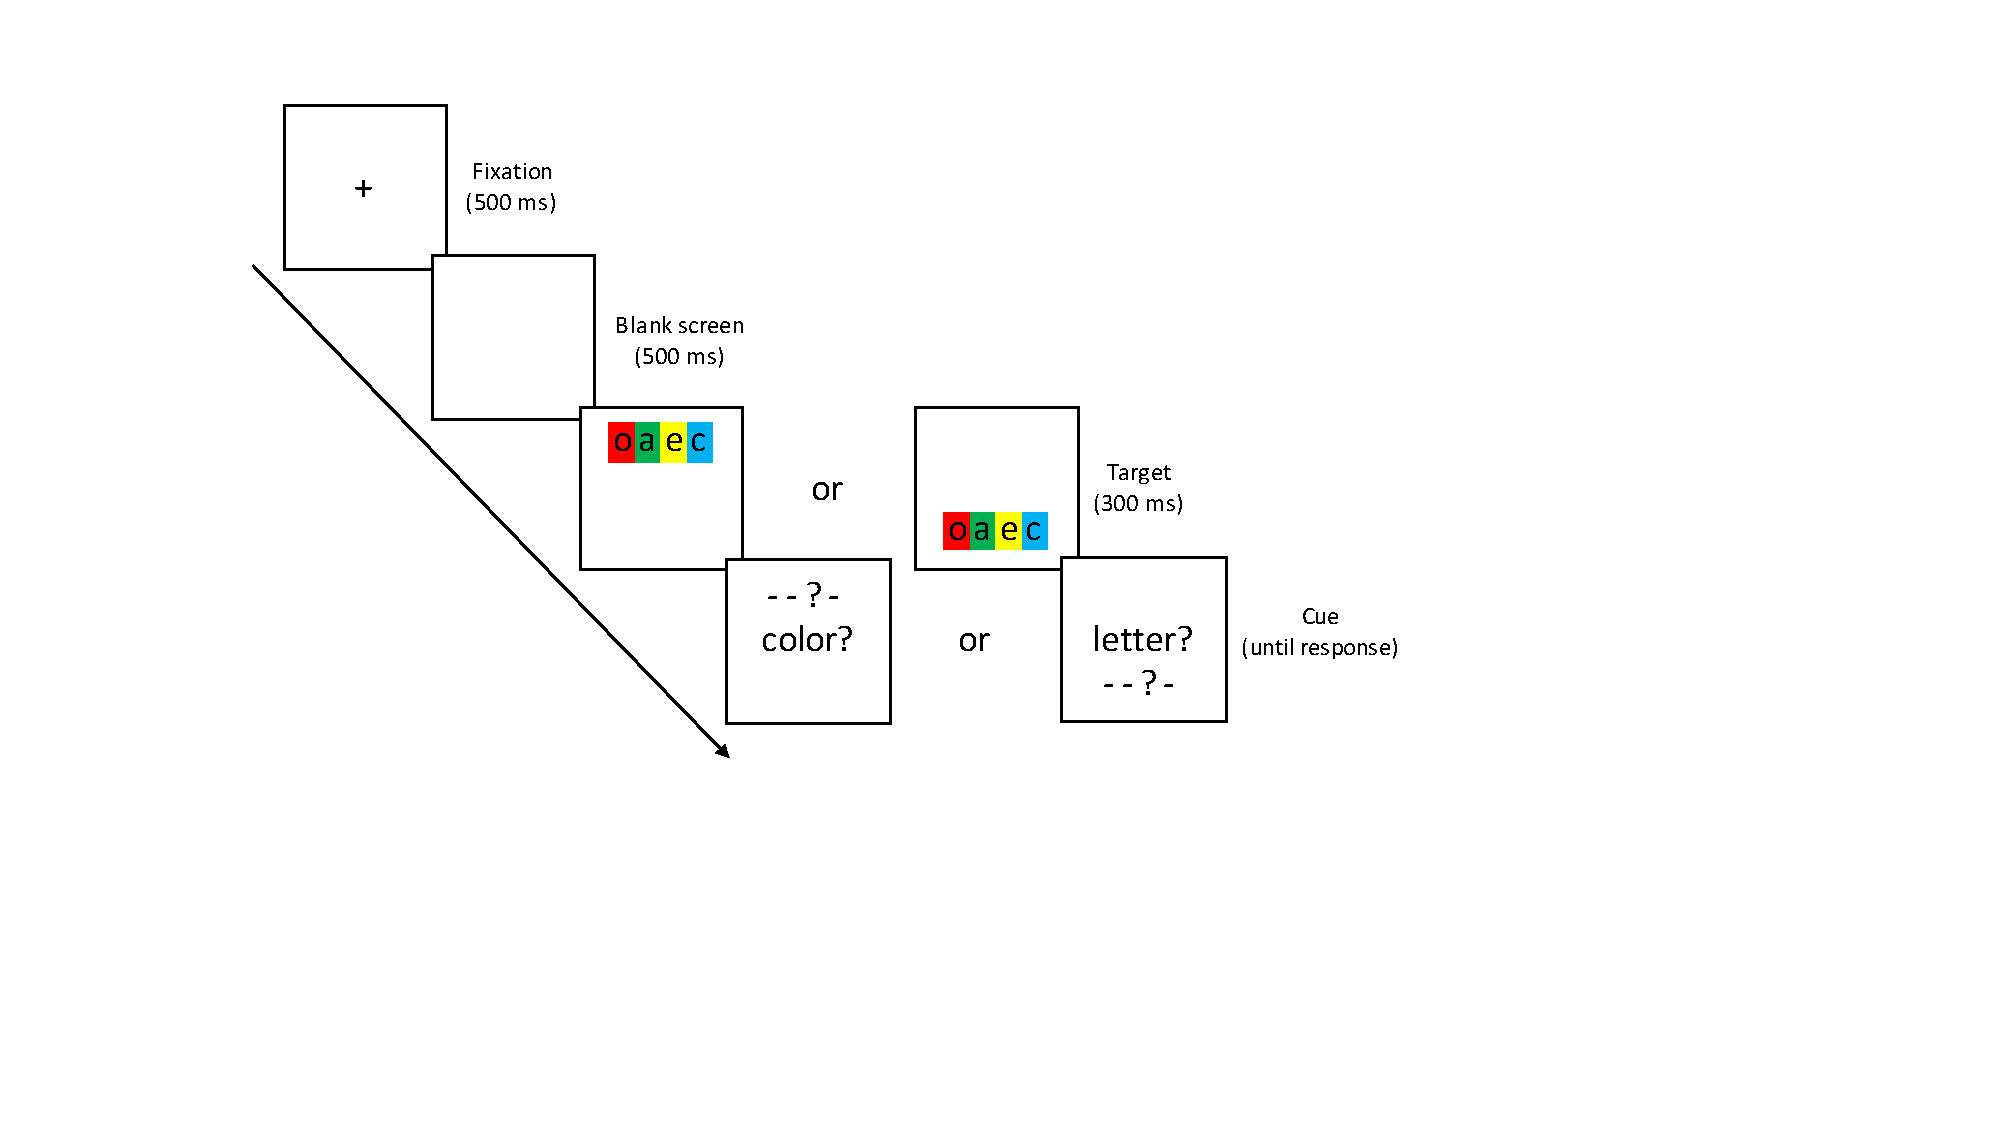
\includegraphics{figures/IC-figure1.pdf}
\caption{\label{fig:figure1}Note that the target could appear above or below the
fixation. The identity cue (\enquote{Color?} or \enquote{Letter?})
always appeared in the center of the screen while the position cue
(\enquote{- - ? -}) always appeared in the same location as the target.
Participants were instructed to report either the letter or color in the
cued position.}
\end{figure}








\subsection{Methods}\label{methods}

\subsubsection{Subjects}\label{subjects}

All subjects were Brooklyn College undergraduate students (approximately
ages 18-22) who participated for course credit. Twenty subjects
completed Experiment 1 and all were included in the analysis.

\subsubsection{Apparatus \& Stimuli}\label{apparatus-stimuli}

All experiments were programmed using LiveCode 7.0. The target stimuli
consisted of four lower-case letters (o, e, c, and a) superimposed on
four colored squares (red, green, blue, and yellow). The relative
positions of letters and colors on each trial were randomly chosen from
all possible letter/color permutations. The background was black and
stimuli were presented either above or below the fixation on a dark gray
rectangle.

The keyboard was labeled to indicate the four letters and four color
responses required. The keys A, S, D, and F were relabeled to A, O, E,
and C respectively; and, the keys H, J, K, and L were relabeled as red,
blue, green, and yellow, respectively.

\subsubsection{Design}\label{design}

Experiment 1 used a 2x2 within-subjects design with cue validity (75\%
vs.~25\%) and task (color identification vs.~letter identification) as
factors. There were 480 trials in Experiment 1. One location (randomly
assigned as above or below the fixation) consisted of 75\% color
identification trials (160 trials) and 25\% letter identification trials
(80 trials) while the other location consisted of 75\% letter
identification trials and 25\% color identification trials. The trial
sequence was randomized and presented in an intermixed fashion for each
subject.

\subsubsection{Procedure}\label{procedure}

Each subject read a brief overview about the stimuli they would be
presented and the types of responses required before signing a consent
form. Subjects were instructed to remember the locations of both the
colors and letters. Immediately following the target stimulus, a cue
would indicate the to-be-identified target, which could be a letter or a
color, located in any of the four positions.

Each trial began with a white fixation-cross presented in the center of
the screen for 500 ms followed by a blank screen for 500 ms. Next, the
target stimulus containing the four letters and four colors appeared for
300 ms followed immediately by the instructions for which stimulus to
identify. The dimension of the to-be-identified stimulus was indicated
by the words \enquote{Letter?} or \enquote{Color?} presented in the
center of the screen and its location was indicated by three dashes and
a question mark (i.e., \enquote{- - ? -}) presented in the same location
as the target stimulus (see Figure \ref{fig:figure1}). For example,
\enquote{Letter?} and \enquote{? - - -} would indicate the letter
located in the first position. No accuracy feedback was given following
a response and the next trial began automatically. A mandatory 30-second
break was given every 120 trials.

\begin{table}[htbp]
\caption{Mean correct color and letter identification response latencies, standard errors, and accuracy rates for all experiments.}
\label{IC_table}
\centering
\begin{tabular}{cccccccccc}
 & & & & \multicolumn{2}{c}{Training Phase} & \multicolumn{4}{c}{Mixed Phase} \\
\cmidrule(rl){5-6}
\cmidrule(rl){7-10}
 & & & & \multicolumn{2}{c}{100\%} & \multicolumn{2}{c}{75\%} & \multicolumn{2}{c}{25\%}  \\
\cmidrule(rl){5-6}
\cmidrule(rl){7-8}
\cmidrule(rl){9-10}
 & & \multicolumn{1}{c}{Task} & & \multicolumn{1}{c}{M} & \multicolumn{1}{c}{SE} & \multicolumn{1}{c}{M} & \multicolumn{1}{c}{SE} & \multicolumn{1}{c}{M} & \multicolumn{1}{c}{SE} \\
\midrule
\multicolumn{2}{l}{\textbf{Exp. 1}}  &   &    &     &     &    &  & & \\
& & \multicolumn{1}{c}{Color} & \multicolumn{1}{c}{ACC} & \multicolumn{1}{c}{-} & \multicolumn{1}{c}{-} & \multicolumn{1}{c}{64.56} & \multicolumn{1}{c}{3.58} & \multicolumn{1}{c}{63.32} & \multicolumn{1}{c}{3.63} \\
& & & \multicolumn{1}{c}{RT} & \multicolumn{1}{c}{-} & \multicolumn{1}{c}{-} & \multicolumn{1}{c}{1611} & \multicolumn{1}{c}{70} & \multicolumn{1}{c}{1606} & \multicolumn{1}{c}{68} \\
& & \multicolumn{1}{c}{Letter} & \multicolumn{1}{c}{ACC} & \multicolumn{1}{c}{-} & \multicolumn{1}{c}{-} & \multicolumn{1}{c}{61.84} & \multicolumn{1}{c}{3.56} & \multicolumn{1}{c}{62.17} & \multicolumn{1}{c}{3.35} \\
& & & \multicolumn{1}{c}{RT} & \multicolumn{1}{c}{-} & \multicolumn{1}{c}{-} & \multicolumn{1}{c}{1824} & \multicolumn{1}{c}{83} & \multicolumn{1}{c}{1858} & \multicolumn{1}{c}{90} \\
\cmidrule(l){2-10}
 &  & & & & & & & & \\
\multicolumn{2}{l}{\textbf{Exp. 2}}  &   &    &     &     &    &  & & \\
& & \multicolumn{1}{c}{Color} & \multicolumn{1}{c}{ACC} & \multicolumn{1}{c}{75.02} & \multicolumn{1}{c}{3.55} & \multicolumn{1}{c}{64.81} & \multicolumn{1}{c}{4.36} & \multicolumn{1}{c}{63.36} & \multicolumn{1}{c}{4.71} \\
& & & \multicolumn{1}{c}{RT} & \multicolumn{1}{c}{1152} & \multicolumn{1}{c}{47} & \multicolumn{1}{c}{1510} & \multicolumn{1}{c}{59} & \multicolumn{1}{c}{1556} & \multicolumn{1}{c}{67} \\
& & \multicolumn{1}{c}{Letter} & \multicolumn{1}{c}{ACC} & \multicolumn{1}{c}{77.11} & \multicolumn{1}{c}{3.23} & \multicolumn{1}{c}{58.31} & \multicolumn{1}{c}{3.4} & \multicolumn{1}{c}{59.09} & \multicolumn{1}{c}{3.88} \\
& & & \multicolumn{1}{c}{RT} & \multicolumn{1}{c}{1309} & \multicolumn{1}{c}{61} & \multicolumn{1}{c}{1707} & \multicolumn{1}{c}{80} & \multicolumn{1}{c}{1711} & \multicolumn{1}{c}{83} \\
\cmidrule(l){2-10}
& & & & & & & & & \\
\multicolumn{2}{l}{\textbf{Exp. 3}}  &   &    &     &     &    &  & & \\
& & \multicolumn{1}{c}{Color} & \multicolumn{1}{c}{ACC} & \multicolumn{1}{c}{79.83} & \multicolumn{1}{c}{3.08} & \multicolumn{1}{c}{67.59} & \multicolumn{1}{c}{4.65} & \multicolumn{1}{c}{56.62} & \multicolumn{1}{c}{4.91} \\
& & & \multicolumn{1}{c}{RT} & \multicolumn{1}{c}{1318} & \multicolumn{1}{c}{61} & \multicolumn{1}{c}{1595} & \multicolumn{1}{c}{58} & \multicolumn{1}{c}{1687} & \multicolumn{1}{c}{62} \\
& & \multicolumn{1}{c}{Letter} & \multicolumn{1}{c}{ACC} & \multicolumn{1}{c}{81.99} & \multicolumn{1}{c}{2.54} & \multicolumn{1}{c}{65.56} & \multicolumn{1}{c}{3.55} & \multicolumn{1}{c}{56.62} & \multicolumn{1}{c}{5.13} \\
& & & \multicolumn{1}{c}{RT} & \multicolumn{1}{c}{1560} & \multicolumn{1}{c}{96} & \multicolumn{1}{c}{1751} & \multicolumn{1}{c}{64} & \multicolumn{1}{c}{1858} & \multicolumn{1}{c}{87} \\
\cmidrule(l){2-10}
 & & & & & & & & & \\
\multicolumn{2}{l}{\textbf{Exp. 4}}  &   &    &     &     &    &  & & \\
& \multicolumn{1}{l}{Trained Context} & \multicolumn{1}{c}{Color} & \multicolumn{1}{c}{ACC} & \multicolumn{1}{c}{67.71} & \multicolumn{1}{c}{4} & \multicolumn{1}{c}{58.4} & \multicolumn{1}{c}{4.34} & \multicolumn{1}{c}{45} & \multicolumn{1}{c}{4.91} \\
& & & \multicolumn{1}{c}{RT} & \multicolumn{1}{c}{1519} & \multicolumn{1}{c}{80} & \multicolumn{1}{c}{1524} & \multicolumn{1}{c}{52} & \multicolumn{1}{c}{1596} & \multicolumn{1}{c}{52} \\
& & \multicolumn{1}{c}{Letter} & \multicolumn{1}{c}{ACC} & \multicolumn{1}{c}{77.81} & \multicolumn{1}{c}{4.14} & \multicolumn{1}{c}{56.04} & \multicolumn{1}{c}{4.52} & \multicolumn{1}{c}{48.12} & \multicolumn{1}{c}{5.39} \\
& & & \multicolumn{1}{c}{RT} & \multicolumn{1}{c}{1686} & \multicolumn{1}{c}{90} & \multicolumn{1}{c}{1625} & \multicolumn{1}{c}{43} & \multicolumn{1}{c}{1620} & \multicolumn{1}{c}{74} \\
\cmidrule(rl){3-10}
& \multicolumn{1}{l}{Reversed Context} & \multicolumn{1}{c}{Color} & \multicolumn{1}{c}{ACC} & \multicolumn{1}{c}{-} & \multicolumn{1}{c}{-} & \multicolumn{1}{c}{56.53} & \multicolumn{1}{c}{4.93} & \multicolumn{1}{c}{51.88} & \multicolumn{1}{c}{4.96} \\
& & & \multicolumn{1}{c}{RT} & \multicolumn{1}{c}{-} & \multicolumn{1}{c}{-} & \multicolumn{1}{c}{1489} & \multicolumn{1}{c}{31} & \multicolumn{1}{c}{1526} & \multicolumn{1}{c}{61} \\
& & \multicolumn{1}{c}{Letter} & \multicolumn{1}{c}{ACC} & \multicolumn{1}{c}{-} & \multicolumn{1}{c}{-} & \multicolumn{1}{c}{52.01} & \multicolumn{1}{c}{4.46} & \multicolumn{1}{c}{47.08} & \multicolumn{1}{c}{5.17} \\
& & & \multicolumn{1}{c}{RT} & \multicolumn{1}{c}{-} & \multicolumn{1}{c}{-} & \multicolumn{1}{c}{1607} & \multicolumn{1}{c}{36} & \multicolumn{1}{c}{1616} & \multicolumn{1}{c}{60} \\
 & & & & & & & & & \\
\bottomrule
\multicolumn{10}{l}{\textit{Note}: RT = Reaction Time (ms);  ACC = Accuracy (\%);  M = Mean; SE = } \\
\multicolumn{10}{l}{Standard Error;  100\%\textbackslash 75\%\textbackslash 25\% = Cue Validity.} \\
\end{tabular}%
\end{table}

\subsection{Results}\label{results}

Overall identification accuracy was fairly low with an average accuracy
of 63\%, though subjects were well above chance (25\%). Given the low
accuracy scores, a response time analysis was inappropriate as nearly
40\% of trials would have been removed from the analysis resulting in
insufficient cell sizes. Furthermore, accuracy was well below ceiling
levels of performance and therefore, would be sensitive to improvements
in performance. Mean RTs and accuracy scores for all experiments are
displayed in Table 1.

Mean accuracy scores for each subject in each condition were submitted
to a repeated-measures ANOVA with cue validity (75\% vs.~25\%) and task
(color identification vs.~letter identification) as factors. Mean
accuracy rates collapsed across subjects are presented in Figure
\ref{fig:figure2}.

Both main effects for cue validity, \(F(1, 19) = 0.21\),
\(\mathit{MSE} = 19.70\), \(p = .654\), \(\hat{\eta}^2_p = .011\), and
task \(F(1, 19) = 0.49\), \(\mathit{MSE} = 152.59\), \(p = .492\),
\(\hat{\eta}^2_p = .025\), were non-significant. Additionally, the
two-way interaction between cue validity and task was also
non-significant, \(F(1, 19) = 0.44\), \(\mathit{MSE} = 28.19\),
\(p = .517\), \(\hat{\eta}^2_p = .022\). Accuracy was not significantly
better for targets presented in their valid versus invalid locations.

\begin{figure}
\centering
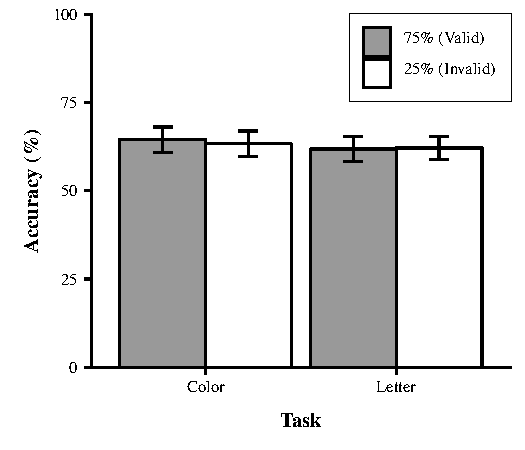
\includegraphics{figures/IC-figure2.pdf}
\caption{\label{fig:figure2}Accuracy scores (\%) for color and letter identification
trials as a function of location cue validity.}
\end{figure}




\subsection{Discussion}\label{discussion}

Experiment 1 failed to demonstrate context-specific control over
priorities for sampling from color vs.~letter dimensions in briefly
presented displays. Specifically, identification performance did not
vary as a function of location cue validity. The absence of contextual
control occurred despite the significant amount of errors made in all
locations. So, although there was an opportunity for adaptive learning
processes to modify attentional priorities based on error signals (in
this case, the subjective appraisals of performance), those processes
did not appear to influence performance. We cannot rule out whether or
not additional practice was necessary for contextual control to develop;
however, it clearly did not develop with amounts of practice sufficient
to produce contextual control in related procedures.

One possibility is that subjects did not attempt to intentionally change
attentional priorities for sampling from color and letter dimensions
between location contexts, and instead adopted a
\enquote{sample-everything} strategy. This strategy would not prioritize
one dimension over another, but would instead involve attempting to
register as many details about both dimensions as possible. If subjects
were employing such an experiment-wide indiscriminate sampling strategy,
then their memory record would not be populated with instances
preserving different attentional priorities between contexts. Experiment
2 was designed to populate the memory record with traces where
attentional priorities were modified between contexts.

\section{Experiment 2}\label{experiment-2}

\begin{figure}
\centering
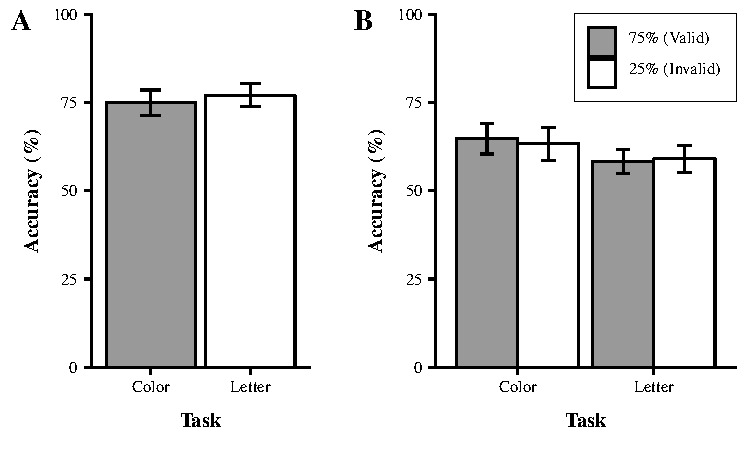
\includegraphics{figures/IC-figure3.pdf}
\caption{\label{fig:figure3}Results for the Training Phase (left) and Mixed Phase
(right) from Experiment 2. Accuracy scores (\%) for color and letter
identification trials as a function of location cue validity.}
\end{figure}





The memory-driven account proposes that attentional processing details
are stored in individual memory traces. Contextual control is then the
result of the cue-driven retrieval and reinstatement of prior
attentional priorities (Crump, 2016; Crump \& Milliken, 2009; Crump et
al., 2006, 2008). One interpretation of the absence of contextual
control in experiment one was the possibility that subjects were
adopting the very same \enquote{sample everything} strategy in both
locations. As a result, the locations may still be operating as
effective cues, but they may be cuing the very same attentional control
settings in both locations. The purpose of Experiment two was to
establish a history of differential attentional processing in each
location. This was achieved by including a blocked practice phase prior
to the mixed trial phase. The practice phase consisted of a block of
trials where a single identification task (e.g., color) was paired
consistently with one location, followed by another block where the
other identification task (e.g., letter) was paired consistently with
the other location. Subjects were informed about the blocked practice
phase and mixed phase experimental structure, but were not informed
about the proportion manipulations.

Proportion congruent designs sometimes include a blocked practice phase
to achieve context-specific attentional control. For example, Lehle and
Hübner (2008) could only demonstrate contextual control over flanker
effects when subjects received blocked practice first (see also Crump,
2016). This is consistent with the memory-driven account which requires
a history of experiences where different attentional priorities were
deployed in different situations. The blocked practice phase would allow
subjects to adopt dimension-specific sampling strategies, and the mixed
phase would allow us to test whether this training is required for
producing contextual control.

\subsection{Methods}\label{methods-1}

\subsubsection{Subjects}\label{subjects-1}

All subjects were Brooklyn College undergraduate students (approximately
ages 18-22) who participated in this study for course credit. Twenty-one
subjects completed Experiment 2.

\subsubsection{Apparatus \& Stimuli}\label{apparatus-stimuli-1}

The apparatus and stimuli were identical to Experiment 1.

\subsubsection{Design}\label{design-1}

The design was similar to Experiment 1 except that subjects completed a
blocked practice phase prior to the mixed phase. Experiment 2, therefore
involved a one-way within-subjects practice phase with task as a factor
(color identification vs.~letter identification) and a separate 2x2
within-subjects design for the mixed phase with cue validity (75\%
vs.~25\%) and task (color identification vs.~letter identification) as
factors. The high-proportion tasks assigned to each location (above or
below the fixation) were randomly assigned across subjects. The
locations assigned to each task in the blocked practice phase were kept
consistent with the validity manipulation in the mixed phase. For
example, if the above location was assigned to color during the block
phase, the same location was assigned to be 75\% color identification in
the mixed phase. Whether the first practice block involved the color or
letter location was randomly assigned across subjects.

There were a total of 512 trials. The first practice block included 128
trials, with all stimuli appearing in one location and requiring only
one identification task. The second block repeated this procedure with
the other location and identification task. The last two blocks (the
mixed phase) consisted of 128 trials each, with 50\% color and letter
identification trials occurring with equal probability above or below
the fixation. As with Experiment 1, one location (randomly assigned as
above or below the fixation) consisted of 75\% color identification
trials (96 trials) and 25\% letter identification trials (32 trials)
while the other location consisted of 75\% letter identification trials
and 25\% color identification trials. The trial sequence was randomized
for each subject.

\subsubsection{Procedure}\label{procedure-1}

The procedure was identical to Experiment 1.

\subsection{Results}\label{results-1}

Mean accuracy scores for each subject in each condition are displayed in
Figure \ref{fig:figure3}. Mean RTs and accuracy scores for all
experiments are displayed in Table 1.

\subsubsection{Training Phase.}\label{training-phase.}

Mean accuracy scores for each subject were submitted to a
repeated-measures ANOVA with task (color identification vs.~letter
identification) as the sole factor. There was no significant difference
between mean accuracy in the color identification block (M = 74.6\%) and
the letter identification block (M = 76.6\%), \(F(1, 20) = 0.29\),
\(\mathit{MSE} = 159.68\), \(p = .597\), \(\hat{\eta}^2_p = .014\).

\subsubsection{Mixed Phase.}\label{mixed-phase.}

Mean accuracy scores for each subject were submitted to a
repeated-measures ANOVA with cue validity (75\% vs.~25\%) and task
(color identification vs.~letter identification) as factors. Both main
effects for cue validity, \(F(1, 20) = 0.04\), \(\mathit{MSE} = 0.01\),
\(p = .847\), \(\hat{\eta}^2_p = .002\) and task, \(F(1, 20) = 1.96\),
\(\mathit{MSE} = 0.03\), \(p = .177\), \(\hat{\eta}^2_p = .089\) were
non-significant. The two-way interaction between cue validity and task
was also non-significant, \(F(1, 20) = 0.46\), \(\mathit{MSE} = 0.01\),
\(p = .505\), \(\hat{\eta}^2_p = .023\). Subjects performed equally well
on the valid and invalidly cued trials.

How performance compared between the mixed and training phases was also
of interest. To address this question, overall accuracy scores from the
mixed and training phases were submitted to a pairwise t-test and found
that subjects performed significantly better in the Training Phase (M =
76\%) than the Mixed Phase (M = 61\%), \(t(20) = -5.38\), \(p < .001\).

\subsection{Discussion}\label{discussion-1}

Experiment 2 again failed to demonstrate context-specific control over
attentional priorities for sampling from color and letter dimensions in
briefly presented displays. As with Experiment 1, in the mixed phase
targets were not better identified on valid versus invalid trials.

However, accuracy was substantially better in the blocked practice phase
than the mixed phase. One interpretation of this finding is that
attentional priorities for sampling from letter vs.~color dimensions can
be set in a preparatory fashion, when subjects know in advance which
dimension will be cued. On this view, our blocked phase would have
successfully created a memory record that would be suitable for
producing contextual control. That is, each subject would have a history
of experiences where they prioritized the color dimension in one
location and the letter dimension in the other. Yet, there was no
evidence of contextual control in the mixed phase.

There are several possibilities for the absence of context-specific
effects. Increased accuracy in the blocked phase may not reflect changes
to attention, but could instead reflect general differences in task
difficulty between blocked and mixed phases. Perhaps contextual control
phenomena do not generalize to our bi-dimensional sampling task.
Finally, it is possible that contextual control can be interfered with
by intentional control. More specifically, even though subjects may have
learned to assign different attentional priorities in each location
during the blocked practice phase, when they were confronted with the
trial-to-trial uncertainty of the upcoming identification task in the
mixed phase, they may have intentionally deployed a
\enquote{sample-everything} strategy, which could have superseded any
contextual influences over setting attentional priorities.

\section{Experiment 3}\label{experiment-3}

Experiment 3 investigated the role of intentions in producing contextual
control. Subjects were made aware of the location-specific proportion
manipulation and explicitly instructed to adopt and maintain
differential attentional strategies in each location. Specifically,
subjects were instructed to attend more to the colors in the color
location and more to the letters in the letter location, as indicated by
the training phase. Importantly, subjects were instructed to maintain
the location-specific attentional priorities in the mixed phase. In this
way, we tested whether or not context-specific differences in
attentional priorities could be set by intentional means

\subsection{Methods}\label{methods-2}

\subsubsection{Subjects}\label{subjects-2}

All subjects were Brooklyn College undergraduate students (approximately
ages 18-22) who participated in this study for course credit. A total of
20 subjects completed Experiment 3.

\subsubsection{Apparatus \& Stimuli}\label{apparatus-stimuli-2}

The apparatus and stimuli were identical to the previous experiments.

\subsubsection{Design}\label{design-2}

The design was identical to Experiment 2.

\subsubsection{Procedure}\label{procedure-2}

The procedure was similar to Experiment 2, however in Experiment 3
subjects were made aware of the proportion manipulation and instructed
to follow explicit strategies consistent with the predictiveness of the
location cue. Specifically, they were instructed to maintain the
strategy of \enquote{attend more to the letters in the letter location}
and \enquote{attend more to the colors in the color location} as defined
by their practice phase. In addition, they were told to do there best
when they were asked to identify a dimension that was inconsistent with
the strategy, but to continue the strategy.

\subsection{Results}\label{results-2}

One concern with adopting this set of instructions was that subjects
would ignore the task cues and always respond with the high-proportion
task response set. For example, when the target display occurred in the
75\% letter location, subjects may ignore the cue that says
\enquote{Color?} and respond with a letter every trial. To determine
which subjects may have adopted this strategy, we calculated the task
accuracy for each subject in each condition. The task accuracy reflects
the proportion of trials where a subject responded with one of the four
appropriate response keys (letters when asked for a letter and colors
when asked for a color) regardless of whether it was the correct
response. Subjects with less than 25\% task accuracy in any condition
were not included in the analysis. This criterion was applied to all
remaining analyses. For Experiment 3, this eliminated three subjects.
Mean task accuracy for the remaining subjects was 96\%.

Mean accuracy scores for each subject in each condition are displayed in
Figure \ref{fig:figure4}. Mean RTs and accuracy scores for all
experiments are displayed in Table 1.

\subsubsection{Training Phase}\label{training-phase}

There was no significant difference between the mean accuracy in the
color identification block (M = 79.8\%) and the letter identification
block (M = 81.9\%), \(F(1, 16) = 0.61\), \(\mathit{MSE} = 64.60\),
\(p = .445\), \(\hat{\eta}^2_p = .037\).

\subsubsection{Mixed Phase}\label{mixed-phase}

Mean accuracy scores for each subject were submitted to a
repeated-measures ANOVA with cue validity (75\% vs.~25\%) and task
(color identification vs.~letter identification) as factors. The
critical main effect of cue validity was significant
\(F(1, 16) = 14.34\), \(\mathit{MSE} = 0.01\), \(p = .002\),
\(\hat{\eta}^2_p = .473\). Additionally, the main effect for task was
non-significant \(F(1, 16) = 0.06\), \(\mathit{MSE} = 0.03\),
\(p = .808\), \(\hat{\eta}^2_p = .004\), and the two-way interaction
between cue validity and task was non-significant \(F(1, 16) = 0.28\),
\(\mathit{MSE} = 0.01\), \(p = .605\), \(\hat{\eta}^2_p = .017\).
Subjects therefore performed better for both letter and color targets on
valid than invalid trials.

\subsection{Discussion}\label{discussion-2}

Experiment 3 successfully demonstrated that subjects can adjust
attentional priorities for sampling from letter versus color dimensions
between contexts in the mixed phase. It is possible that the adjustment
of attentional priorities reflected contextual control processes, but
they could also reflect rapid intentional control. That is, subjects
could simply be following task instructions to deliberately change their
attentional priorities in response to the location context in which a
display occurs.

\begin{figure}
\centering
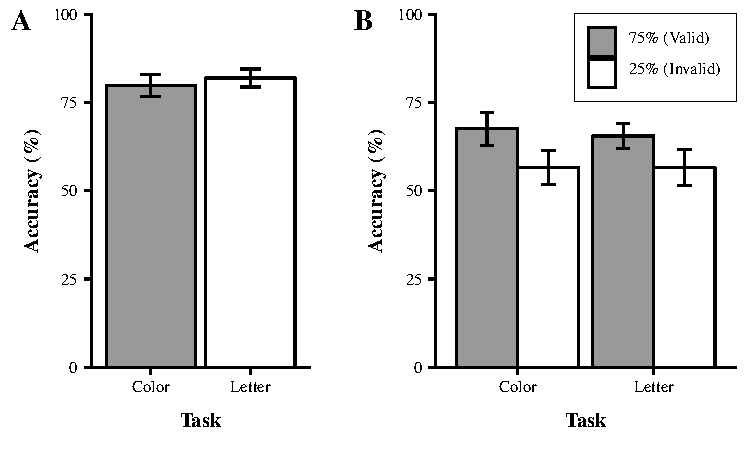
\includegraphics{figures/IC-figure4.pdf}
\caption{\label{fig:figure4}Results for the Training Phase (left) and Mixed Phase
(right) from Experiment 3. Accuracy scores (\%) for color and letter
identification trials as a function of location cue validity.}
\end{figure}





\section{Experiment 4}\label{experiment-4}

Experiment 4 used a process-dissociation type logic (Jacoby, 1991) to
isolate potential automatic and voluntary influences driving the
context-specific effects found in Experiment 3. Like Experiments 2 and
3, Experiment 4 included a blocked practice and a mixed phase. However,
the mixed phase contained two kinds of blocks that were either
consistent or inconsistent with training. In the consistent blocks, the
valid (75\%) locations for color and letter tasks were consistent with
training. In the inconsistent blocks, the valid locations were reversed
from those used in training. Additionally, subjects were instructed
throughout the experiment about which dimension should be attended to in
each location. Subjects were always told which location was valid for
both tasks, and were always instructed to prioritize each task in its
respective predicted location for the current block. If the effects from
Experiment 3 are due solely to volition, then subjects should be able to
adjust their strategies appropriately even when those strategies are
assigned to locations that were inconsistent with training. If on the
other hand, subjects did form associations between location cues and
intentionally set attentional priorities, then reversing the
high-proportion tasks assigned to location contexts should interfere
with context-specific effects by acting against intentional influences.

\subsection{Methods}\label{methods-3}

\subsubsection{Subjects}\label{subjects-3}

All subjects were Brooklyn College undergraduate students (approximately
ages 18-22) who participated in this study for course credit. Twenty-six
subjects completed Experiment 4.

\subsubsection{Apparatus \& Stimuli}\label{apparatus-stimuli-3}

The apparatus and stimuli were identical to the previous experiments.

\subsubsection{Design}\label{design-3}

The design was similar to Experiment 3 except that subjects completed
blocks of trials where the high-proportion locations were reversed. This
involved a practice phase with task as a factor (color identification
vs.~letter identification), and a separate 2x2x2 within-subjects design
for the mixed phase with cued validity (75\% vs.~25\%), task (color
identification vs.~letter identification) and test blocks (trained
context vs.~reversed context) as factors. The high-proportion tasks
assigned to each location (above or below the fixation) were randomly
assigned across subjects. The locations assigned to each high-proportion
task in the blocked practice phase were consistent with the trained
context blocks and reversed in the reversed context blocks.
Additionally, whether the first practice block involved the
high-proportion color or high-proportion letter location was also
randomly assigned across subjects.

There were 480 trials. The first practice block included 48 trials, with
all stimuli appearing in one location and requiring only one
identification task. The second block repeated this procedure with the
other location and other identification task. The mixed phase involved
four blocks of 96 trials with 50\% color and letter identification
trials occurring with equal probability above or below the fixation. One
location (randomly assigned to above or below the fixation) consisted of
75\% color identification trials and 25\% letter identification trials
while the other location consisted of 75\% letter identification trials
and 25\% color identification trials. The first and third blocks were
trained context blocks, in that the locations for the valid trials were
consistent with those during training. The second and fourth blocks were
reversed context blocks, in that the locations for the valid trials were
reversed from those in the training phase. The trial sequence was
randomized for each subject.

\subsubsection{Procedure}\label{procedure-3}

The procedure was similar to Experiment 3, in that subjects were made
aware of the proportion manipulation and instructed to follow explicit
strategies to account for the predictiveness of the location cue.
However, every 96 trials, the prompt would instruct them to reverse
their strategies.

\subsection{Results}\label{results-3}

As with Experiment 3, task accuracy was calculated for each subject and
those with less than 25\% were not included in the analysis.
Accordingly, six subjects were eliminated from the following analysis.
Mean task accuracy for the remaining subjects was 92\%. Mean accuracy
scores for each subject in each condition are displayed in Figure
\ref{fig:figure5}. Mean RTs and accuracy scores for all experiments are
displayed in Table 1.

\subsubsection{Training phase}\label{training-phase-1}

Accuracy was significantly better in the letter identification task (M =
77.8\%) than the letter identification block (M = 67.7\%),
\(F(1, 19) = 10.48\), \(\mathit{MSE} = 97.38\), \(p = .004\),
\(\hat{\eta}^2_p = .356\).

\subsubsection{Mixed phase}\label{mixed-phase-1}

Mean accuracy scores for each subject were submitted to a
repeated-measures ANOVA with cue validity (75\% vs.~25\%), task (color
identification vs.~letter identification) and test blocks (trained
context vs.~reversed context) as factors.

The three-way interaction between cue validity, task, and test blocks
was non-significant, \(F(1, 19) = 1.94\), \(\mathit{MSE} = 0.00\),
\(p = .180\), \(\hat{\eta}^2_p = .093\). However, the critical two-way
interaction between cue validity and test blocks was significant
\(F(1, 19) = 5.25\), \(\mathit{MSE} = 0.01\), \(p = .034\),
\(\hat{\eta}^2_p = .217\), showing that the validity effect was larger
during trained context test blocks compared to reversed context test
blocks. To further analyze the significant two-way interaction, task was
collapsed over and the reversed and trained context conditions were
analyzed separately. A separate analysis of the trained context revealed
significantly higher accuracy on valid (M = 57\%) than invalid (M =
47\%) trials, \(t(19) = 3.34\), \(p = .003\). The analysis of the
reversed context also showed higher accuracy on valid (M = 54\%) than
invalid (M = 50\%) trials, \(t(19) = 2.09\), \(p = .050\).

For the sake of completeness: The two-way interaction between cue
validity and task \(F(1, 19) = 1.00\), \(\mathit{MSE} = 0.01\),
\(p = .329\), \(\hat{\eta}^2_p = .050\), and task and test blocks, ,
were both non-significant. Finally, the main effect for cue validity was
significant, \(F(1, 19) = 9.85\), \(\mathit{MSE} = 0.02\), \(p = .005\),
\(\hat{\eta}^2_p = .341\), and the main effects for both task
\(F(1, 19) = 0.98\), \(\mathit{MSE} = 0.02\), \(p = .335\),
\(\hat{\eta}^2_p = .049\), and test blocks, \(F(1, 19) = 0.00\),
\(\mathit{MSE} = 0.01\), \(p = .991\), \(\hat{\eta}^2_p = .000\), were
non-significant.

\begin{figure}
\centering
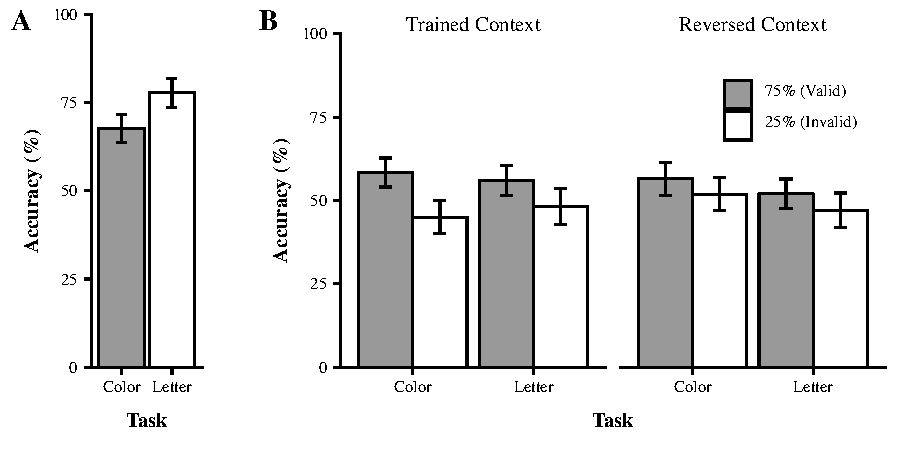
\includegraphics{figures/IC-figure5.pdf}
\caption{\label{fig:figure5}Results for the Training Phase (left) and Mixed Phase
(right) from Experiment 4. Accuracy scores (\%) for color and letter
identification trials as a function of location cue validity.}
\end{figure}





\subsubsection{Block analysis}\label{block-analysis}

Also of interest was whether the validity effects changed over the
course of the experiment. We divided the test trials in half, examining
the validity effects in the first half of the test trials (comprised of
the first trained and reversed context blocks) and the second half
(comprised of the second trained and reversed context blocks). A visual
inspection of the results displayed in Figure \ref{fig:figure6} suggest
a validity effect for the trained context block but not the reversed
context block in the first half, and no validity effects for either the
trained or reversed context blocks in the second half. This result was
confirmed in the following statistical analyses. For the sake of
brevity, only the critical tests are reported.

Mean accuracy scores were submitted to a repeated-measures ANOVA with
test half (first half vs.~second half), cue validity (75\% vs.~25\%),
task (color identification vs.~letter identification), and test block
(trained context vs.~reversed context) as factors. The four-way
interaction was non-significant, \(F(1, 19) = 0.01\),
\(\mathit{MSE} = 0.01\), \(p = .926\), \(\hat{\eta}^2_p = .000\).
However, the critical three-way interaction between test half, test
block, and cue validity was significant, \(F(1, 19) = 7.55\),
\(\mathit{MSE} = 0.02\), \(p = .013\), \(\hat{\eta}^2_p = .284\).

To probe the three-way interaction, each test half (first and second)
was analyzed separately, collapsing over task. Mean accuracy scores for
each test half were submitted to a repeated measures ANOVA with cue
validity (75\% vs.~25\%) and test block (trained context vs.~reversed
context) as factors.

First, we analyzed the first half and found a significant two-way
interaction between cue validity and test block, \(F(1, 19) = 18.27\),
\(\mathit{MSE} = 0.01\), \(p < .001\), \(\hat{\eta}^2_p = .490\).
Further analyses of the simple effects revealed significantly higher
accuracy in the 75\% (valid) trials (M = 57\%) as compared to the 25\%
(invalid) trials (M = 37\%) for the trained context, \(t(19) = 4.62\),
\(p < .001\), and no significant difference between accuracy scores in
the 75\% (valid) and 25\% (invalid) trials for the reversed context,
\(t(19) = 1.62\), \(p = .121\).

An analysis of the second half revealed no significant two-way
interaction between cue validity and test block, . The main effect of
cue validity was also non-significant, \(F(1, 19) = 2.23\),
\(\mathit{MSE} = 0.01\), \(p = .152\), \(\hat{\eta}^2_p = .105\). The
main effect of test block however, was significant, \(F(1, 19) = 8.63\),
\(\mathit{MSE} = 0.01\), \(p = .008\), \(\hat{\eta}^2_p = .312\).

To summarize, we analyzed the first and second halves of the test trials
separately and found a significant validity effect for the trained
context and no validity effect for the reversed context in the first
half of the test trials. For the second half we found no significant
validity effects across both the trained and reverse context test
blocks.

\begin{figure}
\centering
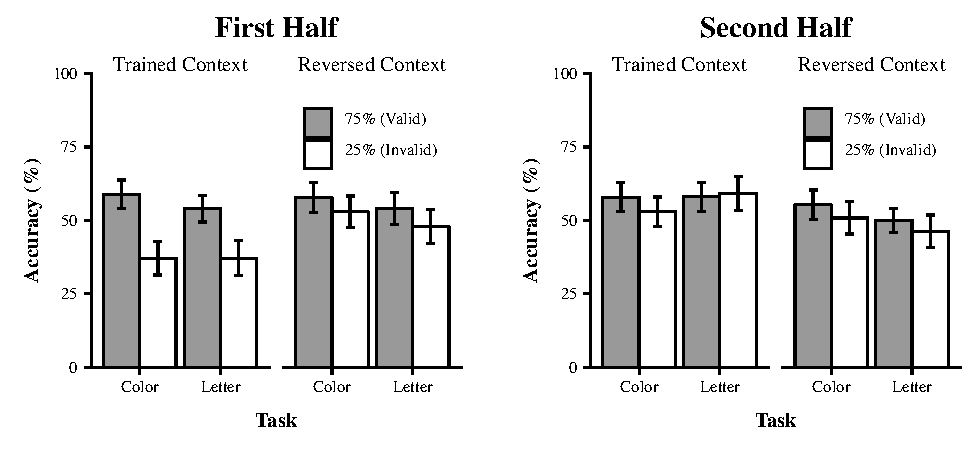
\includegraphics{figures/IC-figure6.pdf}
\caption{\label{fig:figure6}Results from Experiment 4 for the first (left) and second
(right) halves of the Mixed Phase. Accuracy scores (\%) as a function of
task (color vs.~letter), location cue validity (75\% vs.~25\%) and test
blocks (trained context vs.~reversed context)}
\end{figure}






\subsection{Discussion}\label{discussion-3}

The results of Experiment 4 replicate the general findings of Experiment
3 showing that identification accuracy was higher on valid than invalid
trials. The critical finding was that the validity effect depended on
the nature of the test block. The validity effect was larger on trained
context blocks compared to reversed context blocks. Trained context
blocks assigned the 75\% color and 75\% letter task locations to the
same locations used for each task during blocked practice. The reversed
context blocks flipped the assignment with respect to blocked practice.
As a reminder, prior to and during each test block subjects were always
told which location predicted each task. They were also instructed to
attend more to color in the location that predicted the color task, and
more to letters in the location that predicted the letter task. If the
validity effect was entirely driven by a flexible intentional control
process, then we expected that process to produce equivalent validity
effects regardless of whether the test block was consistent or reversed
from training. Instead, we found smaller validity effects in the
reversed context test blocks. One interpretation of this finding is that
the associations between contextual cues and attentional strategies
formed during training interfered with the deployment of intentional
strategies during the reverse context test blocks. On this view, the
results from Experiments 3 and 4 are not due solely to voluntary shifts
in attentional prioritization, but also reflect some contribution of
contextual control over setting of attentional priorities.

We also found significant changes in the validity effects from the first
to second half of the test blocks. Specifically, there was only a
validity effect in the first block of the trained context trials and
there were no significant validity effects for the reversed context
trials in either block. Our purpose in running Experiment 4 was to
determine whether the results from Experiment 3 could be accounted for
solely on the basis of volitional shifts in attentional prioritization.
The block analysis then provides even less support for this idea that
subjects could flexibly shift attentional priorities in the reversed
context blocks because there was no evidence for any validity effect
within each reversed block when analyzed separately. However, our design
consisted of a fixed order of test blocks (trained, reversed, trained,
reversed) and we only found validity effects in the first block. One
possibility is that subjects were unable to continually deploy
instructed strategies. Perhaps subjects lacked motivation to continue
applying the instructed strategies or they were motivated but only had
available resources to apply the effortful strategies for a short period
of time. On this view, subjects could voluntarily shift attentional
priorities but chose not to or were unable to maintain voluntary control
over longer periods. However, we note that accuracy in general increased
across blocks, which suggests that subjects became more motivated to
perform well in the task.

Alternatively, the finding that the validity effects were only evident
in the first test blocks could also reflect some contribution of
contextual control over setting of attentional priorities. It is clear
that in the first test block subjects did adopt the trained attentional
strategy, but then failed to adopt the reversed strategy in the second
block. One interpretation is that training provided the needed
experiential support for enacting the strategy, and when that support
was missing (for the reversed context blocks) strategic control was not
possible. Similarly, the disappearance of the validity effect could be
due to the fact that associations formed during training were
extinguished during the mixed phase which involved many new trial types
that were inconsistent with training. This interpretation fits with
previous findings that effectively applying an attentional strategy for
ignoring a distractor requires experiential learning, or practice with
ignoring the distractor (Vecera, Cosman, Vatterott, \& Roper, 2014). For
example, Cunningham and Egeth (2016) examined whether subjects could
make use of a pre-cue signaling the identity of an upcoming distractor
for the purposes of ignoring the irrelevant feature when it appeared.
They found that subjects learned to ignore distractors that were
preceded by a consistent cue that always signaled the same distracting
feature across trials. However, when the pre-cue signaled different
distracting features across trials participants failed to benefit from
the pre-cue for the purpose of ignoring the signaled distractor. Our
results are similar in that subjects were able to transfer their
learning from the practice blocks to the first test block which was
mostly consistent with training. However, across test blocks attentional
sampling demands became increasingly inconsistent with practice and
prevented transfer of learning from the practice phase to test block
performance.

\section{General Discussion}\label{general-discussion}

In experiment one, one location involved 75\% color and 25\% letter
identification trials and the other involved 75\% letter and 25\% color
identification trials. Despite the fact that location predicted the
likely task on each trial, we found no evidence of contextual control.
Specifically, identification performance on validly cued trials was not
different from invalidly cued trials. The automatic adaptation accounts
posit learning processes sensitive to error- or conflict-driven signals;
however, no evidence of contextual control was found in Experiment 1
despite the poor accuracy that should allow for such learning processes
to operate. One explanation of the absence of contextual control was the
suggestion that subjects adopted a \enquote{sample everything} strategy
on every trial, and learned associations between location contexts and
the attentional priorities assigned by the \enquote{sample everything}
strategy.

In experiment two, the mixed phase was preceded by a blocked training
phase where each identification task was performed consistently in a
particular location. The blocked phase was included to ensure that
subjects had experiences with deploying different attentional priorities
between contexts. We found better identification performance in the
blocked than the mixed phases. However, there was no validity effect in
the mixed phase, indicating no evidence of contextual control. Although
there was evidence that subjects did learn to assign different
attentional priorities in the different contexts during the blocked
practice, this learning apparently failed to transfer to control setting
of attentional priorities in the mixed phase. One reason for the absence
of contextual control in the mixed phase was that subjects again decided
to adopt the \enquote{sample everything} strategy which could have
overridden the ability of contextual cues to set attentional priorities.

In experiment three, we repeated the same design as experiment two, but
made subjects aware of the validity manipulation and gave them
instructions to attend more to color information in the 75\% color
location, and more to letter information in the 75\% letter location.
The major finding was the presence of a validity effect in the mixed
phase, indicating that subjects were capable of assigning different
attentional priorities between locations. However, it remained unclear
whether this effect was mediated by cue-driven or intentional influences
over setting of attentional priorities.

In experiment four, we included new test blocks in the mixed phase where
the valid locations for the color and letter tasks were consistent or
reversed from training. The critical finding was a larger validity
effect when the locations were consistent rather than reversed from
training. Here, the maintenance of voluntary attentional strategies was
impaired when the strategies were inconsistent with the attentional
priorities cued by location contexts established during training. This
finding suggests that the validity effect in the mixed phase was not
entirely driven by a flexible intentional process capable of setting
attentional priorities according to instructions, but also reflects a
contribution from contextual influences that control the setting of
attentional priorities in a cue-driven fashion.

One general aim of the present work was to test guiding principles of
contextual control by using a novel bi-dimensional sampling task. We
found some cases where contextual control was not acquired or expressed
in performance, and some cases where contextual control appeared to
depend on previous experience with deploying different strategies for
setting attentional priorities between contexts. We now turn to a
discussion of the roles of awareness and intention in promoting
contextual control, as well as a number of task differences between our
procedure and previous ones that may explain the presence and absence of
contextual control across our experiments.

Our findings depart from previous work showing that contextual control
develops without awareness and intention. We consider two perspectives
about how our findings relate to previous work. First, we may have found
an exceptional case where contextual control does depend on experiences
with intentionally adopting different attentional priorities in
different contexts. On this view, contextual control can develop with or
without intention, and whether or not contextual control relies on
intention would be task-dependent.

Second, we consider the possibility that prior demonstrations of CSPC
effects did depend on experiences with intentionally adopting different
attentional priorities between contexts. A common finding in Stroop and
flanker variants is that subjects are not aware of the CSPC
manipulation. One interpretation of this finding is that subjects who
were not aware of the manipulation did not intentionally use contextual
cues to adopt different attentional priorities. However, we assume that
subjects were always intentionally controlling attention priorities at
the level of specific items, and that individual stimuli provoke
subjects to adopt particular attentional priorities appropriate to the
stimulus and task at hand. Consider the item-specific strategies adopted
by a subject in CSPC Stroop task who is unaware of the CSPC
manipulation, but who is following instructions to respond to a color
dimension as quickly and accurately as possible. When a congruent item
is presented, subjects may actively assign more priority to the word
dimension because it matches with the correct color response. When an
incongruent item is presented, subjects may actively assign less
priority to the word dimensions because it does not match the correct
color response. In this way, subjects may have intentions for setting
attentional priorities at the item-specific level that can be exercised
on each trial regardless of whether they are aware of the
context-specific proportion congruent manipulation. As a result, the
attentional priorities resulting from intentional control at the
item-level could become associated with the contexts in which items
frequently occur, thereby leading to the development of contextual
control.

In order to entertain the view that intentional control does influence
the acquisition of contextual control across tasks, we also need to
consider discrepancies in the effectiveness of instructional
manipulations. We show that subjects can follow instructions to adopt
context-specific attentional priorities in the bi-dimensional sampling
task. However, similar instructional manipulations were not effective in
a CSPC Stroop task (Crump et al., 2008). Here, subjects were encouraged
to adopt context-specific attentional priorities in response to the
shape context of a target stimulus. Subjects were aware of the CSPC
manipulation and were instructed to adopt context-specific attentional
priorities; nevertheless, no evidence of contextual control was
obtained. One interpretation of this finding is that intentional control
is not sufficient for producing contextual control. However, it remains
unclear whether those subjects could follow the instructions. For
example, in their prime-probe Stroop task the subject was briefly
presented with a word that disappeared before the target color patch was
displayed in one of two shapes. The instruction was to use the shape cue
to rely more or less on the previous word to help with responding to the
color of the target. It is not clear how subjects would attempt to
retrospectively ignore the influence of an already presented word.
Therefore, intentional control may have failed to influence the
acquisition of contextual control in those tasks because subjects were
never engaging in context-specific intentional control to begin with. By
contrast, in the current task the instruction to attend more to the
colors versus the letters may be easier to communicate, more readily
understood, and easier to execute than instructions employed in prior
tasks.

Finally, there are critical differences between our task and those that
have previously demonstrated contextual control. Though the current
study suggests that intentional control may be a pre-requisite for the
acquisition of contextual control, these task differences could
potentially limit the generalizability of our findings and warrant
further discussion.

Contextual control has been observed in several interference tasks where
there is response conflict between target and distractor dimensions. In
contrast, there was no apparent response conflict between our color and
letter dimensions. Some theories of contextual control assume that the
presence of this conflict drives learning and mediates the acquisition
of contextual control (Blais et al., 2012; Botvinick et al., 2001;
Verguts \& Notebaert, 2008, 2009). For example, Crump et al. (2008)
showed no CSPC effects in a Stroop task where subjects named words
rather than colors. If contextual control depends on the presence of
response conflict between target and distractor dimension, then the
absence of contextual control in experiments one and two could be due to
the absence of similar kinds of conflict in our task.

At the same time, we assume that our displays prompted ubiquitous
response competition on each trial. Target displays consisted of four
unique letters and colors and therefore on any given trial, eight
potential responses. Additionally, the total amount of response
competition could have been reduced substantially (from eight to four)
to the extent that contextual cues signaled selective processing of the
dimension that was usually probed in that location. On this view, if the
acquisition of contextual control is strongly related to the size of the
conflict signal, we would have expected rapid learning and strong
evidence for contextual control in our first experiments.

Alternatively, it is possible that the high degree of response conflict
prevented the acquisition of contextual control. Prior work has
demonstrated an absence of contextual control when subjects failed to
attend to contextual information. For example, Crump, Gong, and Milliken
(2006) could only find evidence for contextual control using shape cues
when subjects were given a secondary task that required them to
explicitly attend to the shapes. This suggests that contextual
information may need to be attended to and integrated with target
information in order for contextual control to develop. The high degree
of response conflict in our task may have limited the amount of
attention subjects could direct to the contextual features or caused a
failure in the stimulus-context integration process; both of which could
explain the absence of contextual control in our experiments.

The time-course of stimulus presentation relative to the contextual cues
may also influence the acquisition of contextual control. In our
experiments we always presented the target display simultaneously with
the contextual cue. Simultaneous presentation has been effective in
demonstrating contextual control in Stroop and flanker tasks (Bugg \&
Crump, 2012). In general, prior work has not systematically explored how
the time-course of contextual cueing influences the effectiveness of the
cues. However, Reuss et al. (2014) presented the contextual cue either
prior to or simultaneously with the target and found contextual control
in both cases and Fischer, Gottschalk, and Dreisbach (2014) found
contextual control developed more rapidly when the location-context was
cued prior to the target. We could speculate however, that the
effectiveness of the cue changes as a function of the timing
relationships and it is possible that these changes are task-dependent.
For example, simultaneous presentations may be effective in a Stroop or
flanker task, but ineffective in a bi-dimensional sampling task such as
ours. For this reason, it is possible that the absence of contextual
control in our experiments was due to the fact that we used simultaneous
presentations rather than advance presentations. In general, systematic
investigation of time-course issues in any demonstration of contextual
control is an important topic for future work.

Numerous studies show that attentional priorities for processing
stimulus dimensions can be modulated by contextual cues (e.g., Corballis
\& Gratton, 2003; Crump, 2016; Crump et al., 2006, 2008; Gough et al.,
2014; King et al., 2012). Furthermore, a growing body of literature has
demonstrated that awareness of experimental manipulations such as
dimensional-conflict, proportion of trial-types, and contextual cues,
are not required to produce such effects (e.g., Heinemann et al., 2009;
King et al., 2012; Panadero et al., 2015; Reuss et al., 2014; Sarmiento
et al., 2012). This lack of awareness has suggested that contextual
control can occur independent of a subject's intent. Our findings add to
this body of work and show one situation where intentional setting of
attentional priorities appears to be a pre-requisite for
context-specific control. Our experiments also show that principles from
theories of contextual control such as automatic error-driven learning,
and automatic retrieval of prior instances do not necessarily generalize
across tasks in a straightforward manner.

\newpage

\section{References}\label{references}

\begingroup
\setlength{\parindent}{-0.5in} \setlength{\leftskip}{0.5in}

\hypertarget{refs}{}
\hypertarget{ref-blais_rethinking_2012}{}
Blais, C., Harris, M. B., Guerrero, J. V., \& Bunge, S. A. (2012).
Rethinking the role of automaticity in cognitive control. \emph{The
Quarterly Journal of Experimental Psychology}, \emph{65}(2), 268--276.
Retrieved from
\url{http://www.tandfonline.com/doi/abs/10.1080/17470211003775234}

\hypertarget{ref-botvinick_evaluating_2001}{}
Botvinick, M. M., Braver, T. S., Barch, D. M., Carter, C. S., \& Cohen,
J. D. (2001). Evaluating the demand for control: Anterior cingulate
cortex and conflict monitoring. \emph{Psychological Review},
\emph{108}(3), 624--652. Retrieved from
\url{http://ccpweb.wustl.edu/pdfs/BraverandBarch2001EvaluatingtheDemandforControl.pdf}

\hypertarget{ref-bugg_support_2012}{}
Bugg, J., \& Crump, M. J. (2012). In support of a distinction between
voluntary and stimulus-driven control: A review of the literature on
proportion congruent effects. \emph{Frontiers in Psychology}, \emph{3},
367.
doi:\href{https://doi.org/10.3389/fpsyg.2012.00367}{10.3389/fpsyg.2012.00367}

\hypertarget{ref-bugg_multiple_2008}{}
Bugg, J., Jacoby, L. L., \& Toth, J. P. (2008). Multiple levels of
control in the Stroop task. \emph{Memory \& Cognition}, \emph{36},
1484--1494.
doi:\href{https://doi.org/10.3758/MC.36.8.1484}{10.3758/MC.36.8.1484}

\hypertarget{ref-bundesen_independent_2003}{}
Bundesen, C., Kyllingsbæk, S., \& Larsen, A. (2003). Independent
encoding of colors and shapes from two stimuli. \emph{Psychonomic
Bulletin \& Review}, \emph{10}(2), 474--479. Retrieved from
\url{http://link.springer.com/article/10.3758/BF03196509}

\hypertarget{ref-chun_contextual_2000}{}
Chun, M. M. (2000). Contextual cueing of visual attention. \emph{Trends
in Cognitive Sciences}, \emph{4}(5), 170--178. Retrieved from
\url{http://www.sciencedirect.com/science/article/pii/S1364661300014765}

\hypertarget{ref-chun_contextual_1998}{}
Chun, M. M., \& Jiang, Y. (1998). Contextual cueing: Implicit learning
and memory of visual context guides spatial attention. \emph{Cognitive
Psychology}, \emph{36}, 28--71.
doi:\href{https://doi.org/10.1006/cogp.1998.0681}{10.1006/cogp.1998.0681}

\hypertarget{ref-corballis_independent_2003}{}
Corballis, P. M., \& Gratton, G. (2003). Independent control of
processing strategies for different locations in the visual field.
\emph{Biological Psychology}, \emph{64}, 191--209.
doi:\href{https://doi.org/10.1016/S0301-0511(03)00109-1}{10.1016/S0301-0511(03)00109-1}

\hypertarget{ref-cosman_learned_2013}{}
Cosman, J. D., \& Vecera, S. P. (2013). Learned Control Over Distraction
Is Disrupted in Amnesia. \emph{Psychological Science}, \emph{24}(8),
1585--1590.
doi:\href{https://doi.org/10.1177/0956797613475632}{10.1177/0956797613475632}

\hypertarget{ref-crump_learning_2016}{}
Crump, M. J. (2016). Learning to selectively attend from
context-specific attentional histories: A demonstration and some
constraints. \emph{Canadian Journal of Experimental Psychology/Revue
Canadienne de Psychologie Expérimentale}, \emph{70}, 59--77.
doi:\href{https://doi.org/10.1037/cep0000066}{10.1037/cep0000066}

\hypertarget{ref-crump_contextual_2010}{}
Crump, M. J., \& Logan, G. D. (2010). Contextual control over task-set
retrieval. \emph{Attention, Perception, \& Psychophysics}, \emph{72}(8),
2047--2053. Retrieved from
\url{http://link.springer.com/article/10.3758/BF03196681}

\hypertarget{ref-crump_flexibility_2009}{}
Crump, M. J., \& Milliken, B. (2009). The flexibility of
context-specific control: Evidence for context-driven generalization of
item-specific control settings. \emph{The Quarterly Journal of
Experimental Psychology}, \emph{62}, 1523--1532.
doi:\href{https://doi.org/10.1080/17470210902752096}{10.1080/17470210902752096}

\hypertarget{ref-crump_context-specific_2006}{}
Crump, M. J., Gong, Z., \& Milliken, B. (2006). The context-specific
proportion congruent Stroop effect: Location as a contextual cue.
\emph{Psychonomic Bulletin \& Review}, \emph{13}, 316--321.
doi:\href{https://doi.org/10.3758/BF03193850}{10.3758/BF03193850}

\hypertarget{ref-crump_context-specific_2008}{}
Crump, M. J., Vaquero, J. M., \& Milliken, B. (2008). Context-specific
learning and control: The roles of awareness, task relevance, and
relative salience. \emph{Consciousness and Cognition}, \emph{17},
22--36.
doi:\href{https://doi.org/10.1016/j.concog.2007.01.004}{10.1016/j.concog.2007.01.004}

\hypertarget{ref-cunningham_taming_2016}{}
Cunningham, C. A., \& Egeth, H. E. (2016). Taming the White Bear Initial
Costs and Eventual Benefits of Distractor Inhibition.
\emph{Psychological Science}, \emph{27}(4), 476--485.
doi:\href{https://doi.org/10.1177/0956797615626564}{10.1177/0956797615626564}

\hypertarget{ref-egner_multiple_2008}{}
Egner, T. (2008). Multiple conflict-driven control mechanisms in the
human brain. \emph{Trends in Cognitive Sciences}, \emph{12}, 374--380.
doi:\href{https://doi.org/10.1016/j.tics.2008.07.001}{10.1016/j.tics.2008.07.001}

\hypertarget{ref-eriksen_effects_1974}{}
Eriksen, B. A., \& Eriksen, C. W. (1974). Effects of noise letters upon
the identification of a target letter in a nonsearch task.
\emph{Perception \& Psychophysics}, \emph{16}, 143--149.
doi:\href{https://doi.org/10.3758/BF03203267}{10.3758/BF03203267}

\hypertarget{ref-fischer_context-sensitive_2014}{}
Fischer, R., Gottschalk, C., \& Dreisbach, G. (2014). Context-sensitive
adjustment of cognitive control in dual-task performance. \emph{Journal
of Experimental Psychology: Learning, Memory, and Cognition},
\emph{40}(2), 399.

\hypertarget{ref-gough_control_2014}{}
Gough, A., Garcia, J., Torres-Quesada, M., \& Milliken, B. (2014).
Control of spatial orienting: Context-specific proportion cued effects
in an exogenous spatial cueing task. \emph{Consciousness and Cognition},
\emph{30}, 220--233.
doi:\href{https://doi.org/10.1016/j.concog.2014.09.014}{10.1016/j.concog.2014.09.014}

\hypertarget{ref-heinemann_context-specific_2009}{}
Heinemann, A., Kunde, W., \& Kiesel, A. (2009). Context-specific
prime-congruency effects: On the role of conscious stimulus
representations for cognitive control. \emph{Consciousness and
Cognition}, \emph{18}(4), 966--976. Retrieved from
\url{http://www.sciencedirect.com/science/article/pii/S1053810009001354}

\hypertarget{ref-jacoby_process_1991}{}
Jacoby, L. L. (1991). A process dissociation framework: Separating
automatic from intentional uses of memory. \emph{Journal of Memory and
Language}, \emph{30}(5), 513--541. Retrieved from
\url{http://www.sciencedirect.com/science/article/pii/0749596X9190025F}

\hypertarget{ref-king_priming_2012}{}
King, J. A., Korb, F. M., \& Egner, T. (2012). Priming of control:
Implicit contextual cuing of top-down attentional set. \emph{The Journal
of Neuroscience}, \emph{32}, 8192--8200.
doi:\href{https://doi.org/10.1523/JNEUROSCI.0934-12.2012}{10.1523/JNEUROSCI.0934-12.2012}

\hypertarget{ref-kruschke_alcove:_1992}{}
Kruschke, J. K. (1992). ALCOVE: An exemplar-based connectionist model of
category learning. \emph{Psychological Review}, \emph{99}(1), 22.
Retrieved from \url{http://psycnet.apa.org/journals/rev/99/1/22/}

\hypertarget{ref-kruschke_toward_2001}{}
Kruschke, J. K. (2001). Toward a unified model of attention in
associative learning. \emph{Journal of Mathematical Psychology},
\emph{45}(6), 812--863. Retrieved from
\url{http://www.sciencedirect.com/science/article/pii/S0022249600913543}

\hypertarget{ref-kruschke_attention_2003}{}
Kruschke, J. K. (2003). Attention in Learning. \emph{Current Directions
in Psychological Science}, \emph{12}(5), 171--175.
doi:\href{https://doi.org/10.1111/1467-8721.01254}{10.1111/1467-8721.01254}

\hypertarget{ref-kruschke_models_2010}{}
Kruschke, J. K. (2010). Models of attentional learning. In E. Pothos \&
A. Willis (Eds.), \emph{Formal Approaches in Categorization} (pp.
120--152). Cambridge, UK: Cambridge University Press. Retrieved from
\url{https://scholar.google.com/scholar_lookup?title=Models\%20of\%20attentional\%20learning\&author=J.K.\%20Kruschke\&publication_year=2010\&pages=120-152}

\hypertarget{ref-kyllingsbaek_parallel_2007}{}
Kyllingsbæk, S., \& Bundesen, C. (2007). Parallel processing in a
multifeature whole-report paradigm. \emph{Journal of Experimental
Psychology: Human Perception and Performance}, \emph{33}(1), 64.
Retrieved from \url{http://psycnet.apa.org/journals/xhp/33/1/64/}

\hypertarget{ref-le_pelley_learned_2013}{}
Le Pelley, M. E., Vadillo, M., \& Luque, D. (2013). Learned
predictiveness influences rapid attentional capture: Evidence from the
dot probe task. \emph{Journal of Experimental Psychology: Learning,
Memory, and Cognition}, \emph{39}(6), 1888--1900.
doi:\href{https://doi.org/10.1037/a0033700}{10.1037/a0033700}

\hypertarget{ref-lehle_fly_2008}{}
Lehle, C., \& Hübner, R. (2008). On-the-fly adaptation of selectivity in
the flanker task. \emph{Psychonomic Bulletin \& Review}, \emph{15}(4),
814--818. Retrieved from
\url{http://link.springer.com/article/10.3758/PBR.15.4.814}

\hypertarget{ref-logan_when_1979}{}
Logan, G. D., \& Zbrodoff, N. J. (1979). When it helps to be misled:
Facilitative effects of increasing the frequency of conflicting stimuli
in a Stroop-like task. \emph{Memory \& Cognition}, \emph{7}, 166--174.
doi:\href{https://doi.org/10.3758/BF03197535}{10.3758/BF03197535}

\hypertarget{ref-mackintosh_theory_1975}{}
Mackintosh, N. J. (1975). A theory of attention: Variations in the
associability of stimuli with reinforcement. \emph{Psychological
Review}, \emph{82}(4), 276. Retrieved from
\url{http://psycnet.apa.org/journals/rev/82/4/276/}

\hypertarget{ref-macleod_half_1991}{}
MacLeod, C. M. (1991). Half a century of research on the Stroop effect:
An integrative review. \emph{Psychological Bulletin}, \emph{109}(2),
163. Retrieved from \url{http://doi.apa.org/psycinfo/1991-14380-001}

\hypertarget{ref-mayr_outsourcing_2007}{}
Mayr, U., \& Bryck, R. L. (2007). Outsourcing control to the
environment: Effects of stimulus/response locations on task selection.
\emph{Psychological Research}, \emph{71}(1), 107--116.
doi:\href{https://doi.org/10.1007/s00426-005-0039-x}{10.1007/s00426-005-0039-x}

\hypertarget{ref-milliken_context-specific_2012}{}
Milliken, B., Thomson, D. R., Bleile, K., MacLellan, E., \& Giammarco,
M. (2012). Context-specific control and the Stroop negative priming
effect. \emph{The Quarterly Journal of Experimental Psychology},
\emph{65}(7), 1430--1448.

\hypertarget{ref-moray_theory_1973}{}
Moray, N., \& Fitter, M. (1973). A theory and the measurement of
attention. In S. Kornblum (Ed.), \emph{Attention and Performance IV}.
New York: Academic Press.

\hypertarget{ref-panadero_unconscious_2015}{}
Panadero, A., Castellanos, M. C., \& Tudela, P. (2015). Unconscious
context-specific proportion congruency effect in a stroop-like task.
\emph{Consciousness and Cognition}, \emph{31}, 35--45.
doi:\href{https://doi.org/10.1016/j.concog.2014.09.016}{10.1016/j.concog.2014.09.016}

\hypertarget{ref-posner_facilitation_1975}{}
Posner, M. I., \& Snyder, C. R. R. (1975). Facilitation and inhibition
in the processing of signals. \emph{Attention and Performance V},
669--682.

\hypertarget{ref-reuss_unconscious_2014}{}
Reuss, H., Desender, K., Kiesel, A., \& Kunde, W. (2014). Unconscious
conflicts in unconscious contexts: The role of awareness and timing in
flexible conflict adaptation. \emph{Journal of Experimental Psychology:
General}, \emph{143}(4), 1701--1718.
doi:\href{https://doi.org/10.1037/a0036437}{10.1037/a0036437}

\hypertarget{ref-sarmiento_audiovisual_2012}{}
Sarmiento, B. R., Shore, D. I., Milliken, B., \& Sanabria, D. (2012).
Audiovisual interactions depend on context of congruency.
\emph{Attention, Perception, \& Psychophysics}, \emph{74}(3), 563--574.
doi:\href{https://doi.org/10.3758/s13414-011-0249-9}{10.3758/s13414-011-0249-9}

\hypertarget{ref-schouppe_conscious_2014}{}
Schouppe, N., Ferrerre, E. de, Van Opstal, F., Braem, S., \& Notebaert,
W. (2014). Conscious and unconscious context-specific cognitive control.
\emph{Frontiers in Psychology}, \emph{5}.
doi:\href{https://doi.org/10.3389/fpsyg.2014.00539}{10.3389/fpsyg.2014.00539}

\hypertarget{ref-sperling_information_1960}{}
Sperling, G. (1960). The information available in brief visual
presentations. \emph{Psychological Monographs: General and Applied},
\emph{74}(11), 1--29.
doi:\href{https://doi.org/10.1037/h0093759}{10.1037/h0093759}

\hypertarget{ref-stroop_studies_1935}{}
Stroop, J. R. (1935). Studies of interference in serial verbal
reactions. \emph{Journal of Experimental Psychology}, \emph{18}, 643.
doi:\href{https://doi.org/10.1037/h0054651}{10.1037/h0054651}

\hypertarget{ref-thomson_contextual_2013}{}
Thomson, D. R., \& Milliken, B. (2013). Contextual distinctiveness
produces long-lasting priming of pop-out. \emph{Journal of Experimental
Psychology: Human Perception and Performance}, \emph{39}(1), 202.

\hypertarget{ref-vecera_control_2014}{}
Vecera, S. P., Cosman, J. D., Vatterott, D. B., \& Roper, Z. J. (2014).
The control of visual attention: Toward a unified account.
\emph{Psychology of Learning and Motivation}, \emph{60}, 303--347.
Retrieved from
\url{https://books.google.com/books?hl=en\&lr=\&id=y3spAgAAQBAJ\&oi=fnd\&pg=PA303\&dq=control+of+visual+attention+toward+a+unified+account+vecera\&ots=QAkfy4kJf9\&sig=1rYeI5YUdNFfkpQ9u08-FCtQraM}

\hypertarget{ref-verguts_hebbian_2008}{}
Verguts, T., \& Notebaert, W. (2008). Hebbian learning of cognitive
control: Dealing with specific and nonspecific adaptation.
\emph{Psychological Review}, \emph{115}, 518.
doi:\href{https://doi.org/10.1037/0033-295X.115.2.518}{10.1037/0033-295X.115.2.518}

\hypertarget{ref-verguts_adaptation_2009}{}
Verguts, T., \& Notebaert, W. (2009). Adaptation by binding: A learning
account of cognitive control. \emph{Trends in Cognitive Sciences},
\emph{13}, 252--257.
doi:\href{https://doi.org/10.1016/j.tics.2009.02.007}{10.1016/j.tics.2009.02.007}

\hypertarget{ref-wendt_conflict-frequency_2009}{}
Wendt, M., \& Luna-Rodriguez, A. (2009). Conflict-frequency affects
flanker interference: Role of stimulus-ensemble-specific practice and
flanker-response contingencies. \emph{Experimental Psychology},
\emph{56}(3), 206--217. Retrieved from
\url{http://econtent.hogrefe.com/doi/abs/10.1027/1618-3169.56.3.206}

\hypertarget{ref-wendt_location-specific_2008}{}
Wendt, M., Kluwe, R. H., \& Vietze, I. (2008). Location-specific versus
hemisphere-specific adaptation of processing selectivity.
\emph{Psychonomic Bulletin \& Review}, \emph{15}(1), 135--140. Retrieved
from \url{http://link.springer.com/article/10.3758/PBR.15.1.135}

\endgroup


\end{document}
